\documentclass[conference]{IEEEtran}
\IEEEoverridecommandlockouts
% The preceding line is only needed to identify funding in the first footnote. If that is unneeded, please comment it out.
\usepackage{cite}
\usepackage{amsmath,amssymb,amsfonts}
\usepackage{algorithmic}
\usepackage{graphicx}
\usepackage{textcomp}
\usepackage{xcolor}
\usepackage{float}
\usepackage{multirow}
\usepackage{array}
 \usepackage[numbers]{natbib}
 \usepackage{lipsum}
\def\BibTeX{{\rm B\kern-.05em{\sc i\kern-.025em b}\kern-.08em
    T\kern-.1667em\lower.7ex\hbox{E}\kern-.125emX}}
\begin{document}

\title{Image Segmentation Based on Visual Prompt\\
%{\footnotesize \textsuperscript{*}Note: Sub-titles are not captured in Xplore and
%should not be used}
%\thanks{Identify applicable funding agency here. If none, delete this.}
}

\author{
\IEEEauthorblockN{Mai Duc Minh Huy}
\IEEEauthorblockA{\textit{Faculty of Information and Technology} \\
\textit{VNUHCM University of Science}\\
Ho Chi Minh City, Vietnam \\
minhhuymaiduc@gmail.com}

\and
\IEEEauthorblockN{Chung Tin Dat}
\IEEEauthorblockA{\textit{Faculty of Information and Technology} \\
\textit{VNUHCM University of Science}\\
Ho Chi Minh City, Vietnam \\
chungdatk5@gmail.com}
}                      

\maketitle

\begin{abstract}
	\lipsum[50]
\end{abstract}

\begin{IEEEkeywords}
Segmentation, Online Learning, Representation Learning
\end{IEEEkeywords}

\section{Introduction}
\lipsum[10]

\subsection{Background}
\lipsum[30]

\subsection{Motivation}
\lipsum[30]
\subsubsection{Scientific Significance}
\lipsum[30]
\subsubsection{Practical Significance}
\lipsum[30]
\subsection{Problem Statement}

\begin{figure}[H]
	\centering
	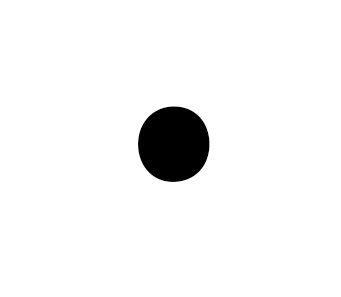
\includegraphics{fig1.png} % Replace with your desired image and size
	\caption{Diagram for Input/ Output here + Framework etc etc} % Add a caption
%	\label{fig:lorem1} % Label for referencing
\end{figure}
% Table 1: Papers, Mechanics, and Methodology
\begin{table*}[t]
	%	\centering
	
	\begin{center} % maximum 0.75
		\caption{Comparison Table - Part 1: Methodology}
		\begin{tabular}{|>{\centering\arraybackslash}p{0.15\textwidth}|>{\centering\arraybackslash}p{0.15\textwidth}|>{\centering\arraybackslash}p{0.15\textwidth}|>{\centering\arraybackslash}p{0.15\textwidth}|>{\centering\arraybackslash}p{0.15\textwidth}|}
			\hline
			\multirow{2}{*}{\textbf{Papers}} & 
			\multirow{2}{*}{\textbf{Mechanics}} & 
			\multicolumn{3}{c|}{\textbf{Methodology}} \\
			\cline{3-5} 
			& &
			\textbf{\centering\textit{Stage 1}} & 
			\textbf{\textit{Stage 2}} & 
			\textbf{\textit{Stage 3}} \\
			\hline
			copy copy copy copy copy copy copy copy copy copy copy copy copy copy copy copy \par copy copy copy copy copy copy copy copy & More table copy$^{\mathrm{a}}$ & & & \\
			\hline
			\multicolumn{5}{l}{$^{\mathrm{a}}$Sample of a Table footnote.}
		\end{tabular}
		\label{tab1}
	\end{center}
\end{table*}
% Table 2: Papers, Performance, Contribution, and Limitation
\begin{table*}[t!]
	\caption{Comparison Table - Part 2: Performance and Analysis}
	\begin{center}
		\begin{tabular}{|>{\centering\arraybackslash}p{0.125\textwidth}|>{\centering\arraybackslash}p{0.125\textwidth}|>{\centering\arraybackslash}p{0.125\textwidth}|>{\centering\arraybackslash}p{0.125\textwidth}|>{\centering\arraybackslash}p{0.125\textwidth}|>{\centering\arraybackslash}p{0.125\textwidth}|}
			\hline
			\multirow{2}{*}{\textbf{Papers}} & 
			\multicolumn{3}{c|}{\textbf{Performance}} &
			\multirow{2}{*}{\textbf{Contribution}} & 
			\multirow{2}{*}{\textbf{Limitation}} \\
			\cline{2-4}
			&
			\textbf{\textit{Data}} & 
			\textbf{\textit{Metric}} &
			\textbf{\textit{Result}} &
			& \\
			\hline
			copy & & & & & \\
			\hline
			\multicolumn{6}{l}{$^{\mathrm{a}}$Sample of a Table footnote.}
		\end{tabular}
		\label{tab2}
	\end{center}
\end{table*}


\subsection{Contribution}
\lipsum[10]


\section{Related Works}

\section{Methodology}

\section{Impletementation \& Experiment}

\section{Conclusion}

\section{Discussion}
\subsection{Limitations}
\subsection{Future Work}\cite{Makarov2022}

\bibliographystyle{IEEEtran} % Or IEEEtranN if using natbib
\bibliography{references}    % Replace 'references' with the name of your .bib file

%\begin{table}[htbp]
%	\caption{}
%	\begin{center}
%		\begin{tabular}{|c|c|c|c|}
%			\hline
%			\textbf{Table}&\multicolumn{3}{|c|}{\textbf{Table Column Head}} \\
%			\cline{2-4} 
%			\textbf{Head} & \textbf{\textit{Table column subhead}}& \textbf{\textit{Subhead}}& \textbf{\textit{Subhead}} \\
%			\hline
%			copy& More table copy$^{\mathrm{a}}$& &  \\
%			\hline
%			\multicolumn{4}{l}{$^{\mathrm{a}}$Sample of a Table footnote.}
%		\end{tabular}
%		\label{tab1}
%	\end{center}
%\end{table}



%
%\begin{table}[htbp]
%	\caption{Comparison Table}
%	\begin{center}
%		\begin{tabular}{|c|c|c|c|c|c|c|c|c|c|}
%			\hline
%			\multirow{2}{*}{\textbf{Papers}} & 
%			\multirow{2}{*}{\textbf{Mechanics}} & \multicolumn{3}{|c|}{\textbf{Methodology}} & 
%			\multicolumn{3}{|c|}{\textbf{Performance}} &
%			\multirow{2}{*}{\textbf{Contribution}} & 
%			\multirow{2}{*}{\textbf{Limitation}} \\
%			\cline{3-8} & &
%			\textbf{\textit{Stage 1}} & 
%			\textbf{\textit{Stage 2}} & 
%			\textbf{\textit{Stage 3}} & 
%			\textbf{\textit{Data}} & 
%			\textbf{\textit{Metric}} &
%			\textbf{\textit{Result}} &
%			&  \\
%			
%			
%			\hline
%			 copy& More table copy$^{\mathrm{a}}$& & & & & & & & \\
%			\hline
%			\multicolumn{4}{l}{$^{\mathrm{a}}$Sample of a Table footnote.}
%		\end{tabular}
%		\label{tab1}
%	\end{center}
%\end{table}
%







\end{document}
